\subsection{Fourierkoeffizienten}
\label{sec:koeffizientenrechnung}
\subsubsection{Rechteckspannung}
Die Funktion der Rechteckspannung \eqref{fig:rechteckspannung} ist
\begin{equation}
  f_\text{r}(t) =
  \begin{cases}
    -A ,  -\frac{\symup{T}}{2} \leq &t \leq 0 \\
     A ,  0 \leq &t \leq \frac{\symup{T}}{2}.
  \end{cases}
\end{equation}
\begin{figure}
  \centering
  \includegraphics[width=\textwidth]{build/recht.pdf}
  \caption{Skizze der Rechteckspannung.}
  \label{fig:rechteckspannung}
\end{figure}
Sie ist ungerade, das heißt $a_n = 0$.
Für $b_n$ ergibt sich mit Gleichung \eqref{eqn:bkoeffizient}
\begin{align}
  b_{n,r} &= \frac{2}{\symup{T}} \left(
  - \! \int_{-\frac{\symup{T}}{2}}^{\, 0} \symup{A} \sin\left(\frac{2\symup{π}n}{\symup{T}}t \right) \, \symup{d}t +
  \int_{\, 0}^{\frac{\symup{T}}{2}} \! \symup{A} \sin\left(\frac{2\symup{π}n}{\symup{T}}t \right) \, \symup{d}t
  \right) \\
  &= \frac{\symup{A}}{\symup{π}n}\left(1-\cos(-\symup{π}n)-\cos(\symup{π}n)+1\right) \\
  &= \frac{2\symup{A}}{\symup{π}n}(1-\cos(\symup{π}n)) \\
  &= \frac{2\symup{A}}{\symup{π}n}(1-(-1)^n).
\end{align}
Damit folgt
\begin{equation}
  b_{n,r} =
  \begin{cases}
    0 , & \text{n gerade} \\
    \frac{4\symup{A}}{\symup{π}n} , & \text{n ungerade.}
    \label{eqn:rechteckko­ef­fi­zi­ent}
  \end{cases}
\end{equation}

\subsubsection{Dreieckspannung}
Die Dreieckspannung \eqref{fig:3eckspannung} wird mit einer geraden Funktion dargestellt;
\begin{equation}
  f_\text{d}(t) =
  \begin{cases}
    - \frac{4\symup{A}}{\symup{T}} t - \symup{A} &, - \frac{\symup{T}}{2} \leq t \leq 0 \\
      \frac{4\symup{A}}{\symup{T}} t - \symup{A} &, 0 \leq t \leq \frac{\symup{T}}{2}.
  \end{cases}
\end{equation}
\begin{figure}
  \centering
  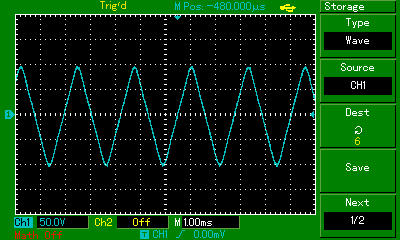
\includegraphics[width=\textwidth]{build/dreieck.pdf}
  \label{fig:3eckspannung}
  \caption{Skizze der Dreieckspannung.}
\end{figure}
Für $b_n$ ergibt sich damit 0.
$a_n$ wird nach \eqref{eqn:akoeffizient} bestimmt,
dafür wird das Integral aufgeteilt.
\begin{align}
  a_{n,d}
  &= - \frac{2}{\symup{T}} \int_{\frac{-\symup{T}}{2}}^{\, 0} \left( \frac{4\symup{A}}{\symup{T}} t + \symup{A} \right) \cos\left(\frac{2\symup{π}n}{\symup{T}}t \right) \, \symup{d}t
     + \frac{2}{\symup{T}} \int_{\, 0}^{\frac{\symup{T}}{2}}  \left( \frac{4\symup{A}}{\symup{T}} t - \symup{A} \right) \cos\left(\frac{2\symup{π}n}{\symup{T}}t \right) \, \symup{d}t \\
  \intertext{Es wird jeweils mit partieller Integration gelöst.}
  &= - \frac{2}{\symup{T}} \left[ \left(\frac{4\symup{A}t}{\symup{T}} + \symup{A}\right) \frac{\symup{T}}{2\symup{π}n} \sin\left(\frac{2\symup{π}n}{\symup{T}}t \right)\right]_{-\frac{\symup{T}}{2}}^0
     - \frac{2\symup{A}}{\symup{π}^2 n^2} \cos\left(\frac{2\symup{π}n}{\symup{T}}t \right) \bigg|_{-\frac{\symup{T}}{2}}^{\, 0} \\
  & + \frac{2}{\symup{T}} \left[ \left(\frac{4\symup{A}t}{\symup{T}} - \symup{A}\right) \frac{\symup{T}}{2\symup{π}n} \sin\left(\frac{2\symup{π}n}{\symup{T}}t \right)\right]_0^{\frac{\symup{T}}{2}}
     + \frac{2\symup{A}}{\symup{π}^2 n^2} \cos\left(\frac{2\symup{π}n}{\symup{T}}t \right) \bigg|_0^{\frac{\symup{T}}{2}} \\
  &= - \frac{\symup{A}}{\symup{π}n} \sin(-\symup{π}n)
     - \frac{2\symup{A}}{\symup{π}^2 n^2} \left(1 - \cos(-\symup{π}n)\right)
     + \frac{\symup{A}}{\symup{π}n} \sin(\symup{π}n)
     + \frac{2\symup{A}}{\symup{π}^2 n^2} \left(\cos(-\symup{π}n) - 1\right) \\
  \intertext{Mit $\sin(\symup{π}n) = 0 \; \forall n \! \in \! \symbb{N}$ und $\cos(\symup{π}n) = \cos(-\symup{π}n)$:}
  &= \frac{4\symup{A}}{\symup{π}^2 n^2} \left(\cos(\symup{π}n) - 1\right) \\
  &= \frac{4\symup{A}}{\symup{π}^2 n^2} \left((-1)^n -1\right).
\end{align}
Es ergibt sich
\begin{equation}
  a_{n,d} =
  \begin{cases}
    0 , & \text{n gerade} \\
    \frac{8 \symup{A}}{\symup{π}^2 n^2} , & \text{n ungerade.}
    \label{eqn:dreieckko­ef­fi­zi­ent}
  \end{cases}
\end{equation}

\subsubsection{Sägezahnspannung}
\begin{figure}
  \centering
  \includegraphics[width=\textwidth]{build/saege.pdf}
  \caption{Skizze der Sägezahnspannung.}
  \label{fig:sägezahnspannung}
\end{figure}

Die Sägezahnspannung \eqref{fig:sägezahnspannung} wird, als ungerade Funktion, mit
\begin{equation}
  f_\text{s} = \frac{2\symup{A}}{\symup{T}}t,\; \; -\frac{\symup{T}}{2} \leq t \leq \frac{\symup{T}}{2}
\end{equation}
bestimmt.
Wie bei der Rechteckspannung ist $a_n =0$ und $b_n$ wird nach \eqref{eqn:bkoeffizient} berechnet.
\begin{align}
  b_{n,s}
  &=   \frac{2}{\symup{T}} \int_{-\frac{\symup{T}}{2}}^{\frac{\symup{T}}{2}} \frac{2\symup{A}}{\symup{T}}t \sin\left(\frac{2\symup{π}n}{\symup{T}}t \right) \, \symup{d}t \\
  &= - \frac{2\symup{A}}{\symup{Tπ}n} \left[t \cos\left(\frac{2\symup{π}n}{\symup{T}}t \right) \right]_{-\frac{\symup{T}}{2}}^{\frac{\symup{T}}{2}}
     + \frac{\symup{A}}{\symup{π}^2 n^2} \sin\left(\frac{2\symup{π}n}{\symup{T}}t \right) \bigg|_{-\frac{\symup{T}}{2}}^{\frac{\symup{T}}{2}} \\
  &= - \frac{2\symup{A}}{\symup{π}n} \cos(\symup{π}n) \\
  &= - \frac{2\symup{A}}{\symup{π}n}(-1)^n \\
  b_{n,s}
  &=   \frac{2\symup{A}}{\symup{π}n}(-1)^{n + 1}.
  \label{eqn:saegekoeffizient}
\end{align}
